\beginsong{Ein stolzes Schiff}[
    txt={Heinrich Schacht},
    txtjahr={1855},
    mel={Erich Schmeckenbecher (Zupfgeigenhansel)},
    meljahr={1978}, 
    pfii={96}, 
    bo={105}, 
    gruen={185}, 
    siru={68},
    tonspur={244}, 
]

\beginverse
\endverse
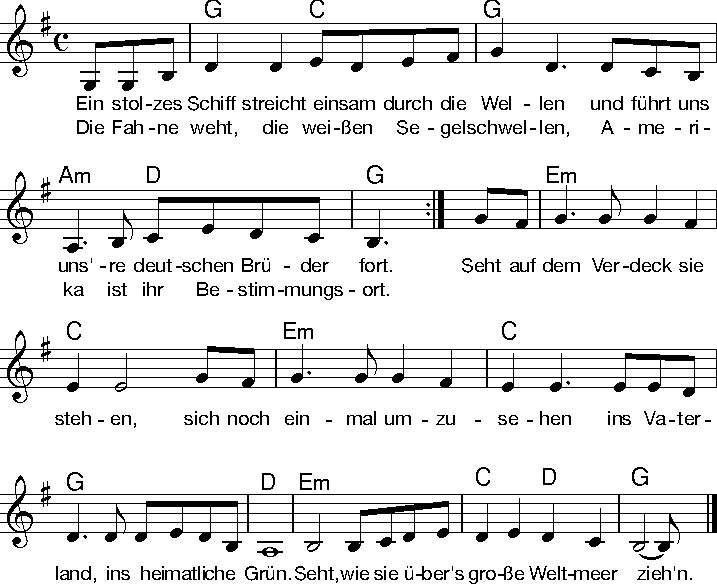
\includegraphics[draft=false, width=1\textwidth]{Noten/Lied033a.pdf}	

\beginverse
Sie zieh'n da\[G]hin auf \[C]blauen Meeres\[G]wogen.
Warum ver\[Am]lassen \[D]sie ihr Heimat\[G]land?
Man hat sie \[G]um ihr \[C]Leben schwer be\[G]trogen,
die Armut \[Am]trieb sie \[D]aus dem Vater\[G]land.
Schauet \[Em]auf, ihr Unter\[C]drücker,
schauet \[Em]auf, ihr Volksbe\[C]trüger,
seht eure \[G]besten Arbeitskräfte \[D]flieh'n,
\[Em]seht, wie sie über's \[C]große \[D]Weltmeer \[G]zieh'n.
\endverse

\beginverse
Sie zieh'n ^dahin, wer ^wagt sie noch zu ^fragen?
Warum ver^lassen ^sie ihr Heimat^land?
Oh, armes ^Deutschland, wie ^kannst du es er^tragen,
dass deine ^Brüder werden ^so ver^bannt?
Was sie ^hofften, hier zu ^gründen,
suchen ^sie dort drüben zu ^finden.
D'rum ziehen ^sie von deutschem Boden ^ab
und ^finden in A^meri^ka ihr ^Grab.
\endverse

\beginverse
Ein stolzes ^Schiff streicht ^einsam durch die ^Wellen,
es führt uns ^uns're ^deutschen Brüder ^fort!
Die Flagge ^weht, die ^weißen Segel ^schwellen,
Ameri^ka ist ^der Bestimmungs^ort.
Seht auf ^dem Verdeck sie ^stehen,
sich noch ^einmal anzu^sehen,
das Vater^land, das heimatliche ^Grün,
^seht, wie sie über's ^große ^Weltmeer ^zieh'n.
\endverse

\endsong

\beginscripture{}
Vermutlich geht das Lied auf die Jahre 1848/49 zurück, als, durch wirtschaftliche Not und politischen Druck gezwungen, Zehntausende von Bauern, Handwerkern und Arbeitern nach Amerika auswanderten. Die Folksänger Schmeckenbecher und Fritz (bekannt unter dem Namen Zupfgeigenhansel) entdeckten den unvollständigen, anonymen Text im Deutschen Volksliedarchiv in Freiburg und ergänzten in sinngemäß. Erst 1995 wurde das vollständige Lied mit seiner ursprünglichen, heute kaum noch gesungenen Melodie gefunden.
\endscripture
